\documentclass[11pt]{article}
\usepackage[margin=0.75in]{geometry}            % See geometry.pdf to learn the layout options. There are lots.
\geometry{letterpaper}                                  % ... or a4paper or a5paper or ... 
%\geometry{landscape}                           % Activate for rotated page geometry
%\usepackage[parfill]{parskip}                  % Activate to begin paragraphs with an empty line rather than an indent
\usepackage{graphicx}                           % Use pdf, png, jpg, or eps§ with pdflatex; use eps in DVI mode
                                                                % TeX will automatically convert eps --> pdf in pdflatex                
\usepackage{amssymb}
\usepackage{upquote}
\usepackage{subcaption} % for side-by-side figures
\usepackage{wrapfig} % for wrapping figures around text
\usepackage{lipsum} % for wrapping figures around text
\usepackage{float}
%-----------------------------------------------------------------------------
% Special-purpose color definitions (dark enough to print OK in black and white)
\usepackage{color}
% A few colors to replace the defaults for certain link types
\definecolor{orange}{cmyk}{0,0.4,0.8,0.2}
\definecolor{darkorange}{rgb}{.71,0.21,0.01}
\definecolor{darkgreen}{rgb}{.12,.54,.11}
%-----------------------------------------------------------------------------
% The hyperref package gives us a pdf with properly built
% internal navigation ('pdf bookmarks' for the table of contents,
% internal cross-reference links, web links for URLs, etc.)
\usepackage{hyperref}
\hypersetup{pdftex, % needed for pdflatex
  breaklinks=true, % so long urls are correctly broken across lines
  colorlinks=true,
  urlcolor=blue,
  linkcolor=darkorange,
  citecolor=darkgreen
}


\title{Wireless Sensor Network Project\\
  Stat 222, Spring 2016}

\author{
  Mengfei Jiang\\
  \url{https://github.com/berkeley-stat222/MengfeiJiang-work}
}


\begin{document}
\maketitle

\abstract{Recent development in wireless sensors has advanced research on microclimate surrounding a large physical volume. A recent study recorded 44 days in the life of a 70-meter-tall interior redwood tree, at a density of every 5 minutes in time and every 2 meters in space, measuring air temperature, humidity and photosynthetically active solar radiation. The report describes a different method to clean and analyze the same multi-dimensional dataset collected by the sensor network from the original paper.}


\section{Introduction}

The paper~\cite{tolle2005macroscope, yang2003redwoods} describes the study of the microclimate surrounding an interior tree within a coastal redwood forest by use of a wireless sensor network deployed over the large organism. Without discussion of hardware and software architecture as well as the deployment methodology as detailed in the paper, this report focuses on the analysis of the same dataset by means of a different methodology in data cleaning, outlier rejection, data exploration, among others to present the variation in spatial and temporal dynamics. The employed methodology is explained in Section 2, with the main findings presented in Section 4. Section 3 discusses the effectiveness of some figures in addressing questions in the original paper, discovers potential room for improvement and speicifies possible alternatives.


\section{The Data}
The entire dataset contains information on two trees, interior and edge, collected over a period with the most dynamic microclimatic variation starting from April 27th 2004 at 5:10pm to June 10th 2014 at 2:00pm by a node network, with four sensors on each node measuring air temperature, relative humidity (RH), direct photosynthetically active solar radiation (incident PAR), and reflected PAR respectively. The readings were taken every 5 minutes at a height ranging from 15m to 70m with a roughly 2-meter spacing between nodes, which were mainly deployed within 0.1-1.0m to the west side of the trunk to capture the microclimatic trends that affected the tree directly while under protection of a thicker canopy against direct environmental effects. Several nodes were also deployed outside the angular and radial range to monitor the immediate vicinity of the environment.

\subsection{Data Collection}
The data were collected from two systems, the TASK system and the local data logging system. The TASK system provides a query-based framework linking the sensor network to a database running on a gateway. Data were firstly stored in a local database to the gateway and then transmitted to another offsite database TinyDB, from which the network data could be queried automatically every 5 minutes throughout the period. On the other hand, the local data logging system existed as a backup of network failure when no data were fetched from TinyDB. The data logger recorded every reading taken by the sensor on each query until the 512KB memory was full. The net dataset and the log datased correspond to the two data collection systems respectively. \\
The two collection systems turned out to be useful. The network data were missed for two periods, the first being the 2-week period from the start to May 7th 6:24pm due to the gateway outage and the second being the week post June 2nd due to periodic data downloading. On the other hand, the log data is not complete from May 26th onwards due to memory fill-up of the data loggers. The intersection of the two datasets identified by the combination of measurement time (\textit{epoch}) and node id (\textit{nodeid}) accounts for roughly 32\% of the log data and 84\% of the net data.\\
Hence, finding a clean way to combine the two datasets post memory fill-up in order to obtain a complete picture of the microclimatic dynamics surrounding the tree is the best one can do, even though the combined dataset might still miss some data points lost in the data collection process in the first place. The detailed method is explained in the next subsection.

\subsection{Data Cleaning}
Data cleaning is best summarized into two parts. The log dataset and the net dataset were first individually checked for variable ranges and number of entries before being combined together. Outliers in the dataset were then removed from the dataset. 

\subsubsection{Dataset Combination and Pre-Processing}
\label{subsubsec:preprocess}
The log and the net dataset were combined based on the theoretically unique combination of $epoch$ and $nodeid$, and the data collected during the week from June 3rd to June 10th were discarded. The first entry of each unique key combination was preserved in case of duplicates in either dataset. The last week data were discarded to avoid analytics bias caused by the fact that only data on the three nodes 42, 127 and 197 were preserved due to gateway failure and data logger memory exhaustion. The data on the three nodes account for around 1.58\% of the original log data. Besides, NA values for the 4 variables, air temperature, humidity, incident PAR and reflected PAR coincide in the dataset, and the corresponding entries were hence all deleted. Then, the tree type information ($edge$ or $interior$) was appended by a merge from the node location dataset. Only the interior tree was the primary focus of the study and hence the data on the edge tree were all discarded. The data from nodes outside the deployment envelope ($>$1m from the trunk), with RH readings beyond the normal 0-100\% range, or with negative adjusted humidity readings were also discarded.


\paragraph{Voltage conversion}
Voltage measures in the net dataset were at 200 level, whereas those in the log within the normal 2 - 3 range. The conversion of the voltage measure in the net to that in the log was calibrated by a simple linear regression with an $R^2$ of 0.9961 after removing a constant voltage reading of 1023 from node 134, 135, 141 and 145, and the graph is shown by Figure~\ref{fig:voltConversion}. The relationship is almost definite and is sufficient for the purpose of outlier rejection in a later stage albeit a slight upward bias.
\begin{figure}[here]
  \centering
    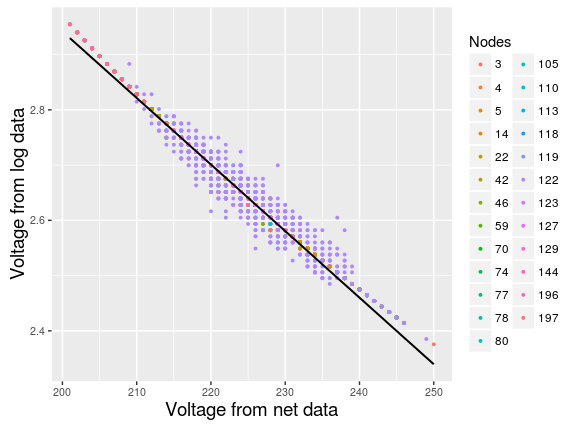
\includegraphics[width=0.5\textwidth]{../figures/voltConversion.png}
  \caption{Net-to-Log voltage conversion}
  \label{fig:voltConversion}
\end{figure}


\paragraph{Epoch conversion}
The simple time conversion task was complicated by the fact that the $result\_time$ was wrongly recorded in the original dataset. In the original net dataset, the epoch 2812 corresponded to the actual time 18:25:00 on May 7th, and hence the epoch 2 was deduced to correspond to 00:05:00 on April 28th. A plot of the incident PAR on May 1st revealed a serious problem: the solar radiation only showed up from around 14:00:00 to after midnight, as shown in Figure ~\ref{fig:wrongTimePAR}. After comparison with the plot in the original paper, it was deduced the epoch 2 should correspond to the actual time 17:15:00 on April 27th, and that all the rest epochs should be adjusted this way. The Figure ~\ref{fig:correctTimePAR} shows the same day incident PAR under the adjusted time. This conversion was ascertained by the annotation in Figure 4 in the original paper specifying the correspondance of epoch 1062 to time 9:35am on May 1st.
\begin{figure}[here]
\centering
\begin{subfigure}{.5\textwidth}
  \centering
  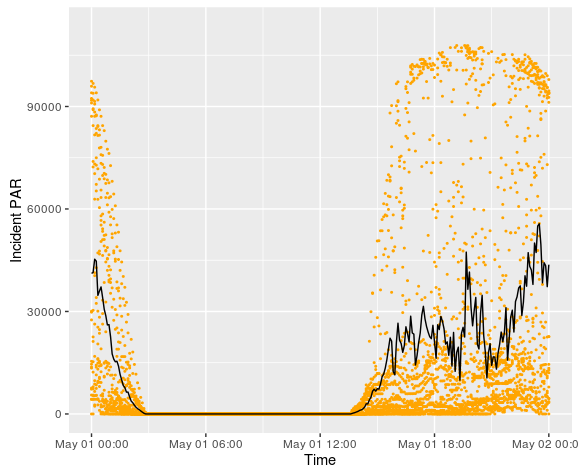
\includegraphics[width=.85\linewidth]{../figures/wrongTimePAR.png}
  \caption{In wrong time}
  \label{fig:wrongTimePAR}
\end{subfigure}%
\begin{subfigure}{.5\textwidth}
  \centering
  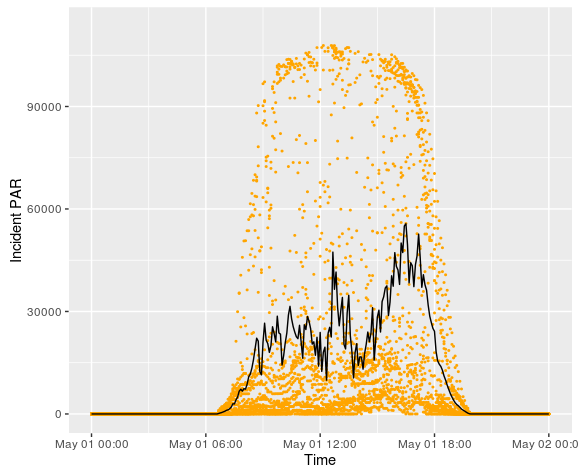
\includegraphics[width=.85\linewidth]{../figures/correctTimePAR.png}
  \caption{In correctly adjusted time}
  \label{fig:correctTimePAR}
\end{subfigure}
\caption{Temporal trend of incident PAR on May 1st, 2004}
\end{figure}

\subsubsection{Outlier Rejection}
A different outlier rejection methodology from that in the original paper was taken to ensure an unbiased clean dataset for further analysis. The paper simply set a hard criteria of rejecting data points with voltage readings beyond the range of 2.4 volts to 3 volts, and claimed that the beyond-range data points were those with abnormal readings in the primary variables of interest, namely air temperature, relative humidiy, incident PAR, and reflected PAR. However, this is not necessarily true. \\
To get a sense of the distribution of the voltage readings, Figure~\ref{fig:boxVoltNode} plots the boxplots of all the node voltage readings side by side within the range of 2 volts to 3 volts. Firstly, those readings for node 134 and 141 are missed because of their negative readings outside the plotting range, and are shown in Figure~\ref{fig:voltDate2}. Secondly, node 78 and node 138 are much more skewed to lower readings than the rest. Less attention is placed on the higher readings because the maximum reading of 3.03 volts indicates nothing but a node working under normal battery conditions. Thirdly, node 109 is much more concentrated than the rest, which might be due to a truly smaller variance or a smaller number of readings obtained as a result of a much shorter battery life. \\
Following the methodology described in the paper, all data points from node 134, 141, and some data points from node 78 and 138 should be removed due to potentially problematic readings of the primary variables. Figure~\ref{fig:tempDate} shows the temperature readings of the 5 nodes against the others, and partially disapproves the claim by the paper. In the case of node 138 whose voltage readings fell below 2.4 volts near June 2nd, all its temperature readings were within the normal range of its peers, and so did its readings of the other variables. In the case of node 134, its readings over the life were normal compared to the peers, and hence should not be removed. So is node 138. Only part of the data from the node 141 should be removed, roughly starting after its last reading in the log data set when the data logger memory filled up. The same applies to node 78. In the case of node 109, although most of its voltage readings were well below the rest as shown by Figure~\ref{fig:voltDate1}, all the temperature readings were similar to the rest, albeit a shorter life.
\begin{figure}[here]
  \centering
  \begin{subfigure}{.5\textwidth}
    \centering
      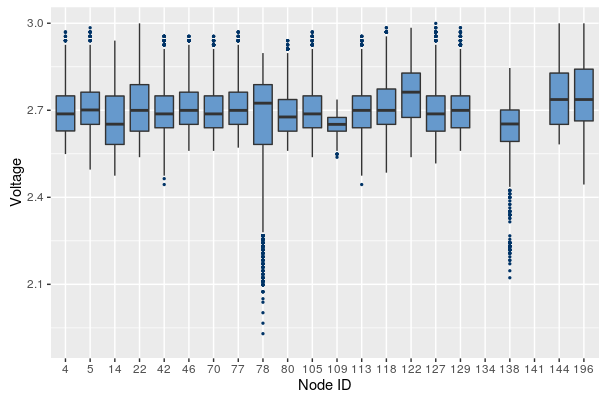
\includegraphics[width=0.9\linewidth]{../figures/box_volt_node.png}
    \caption{Voltage distribution of interior nodes}
    \label{fig:boxVoltNode}
  \end{subfigure}%
  \begin{subfigure}{.5\textwidth}
    \centering
      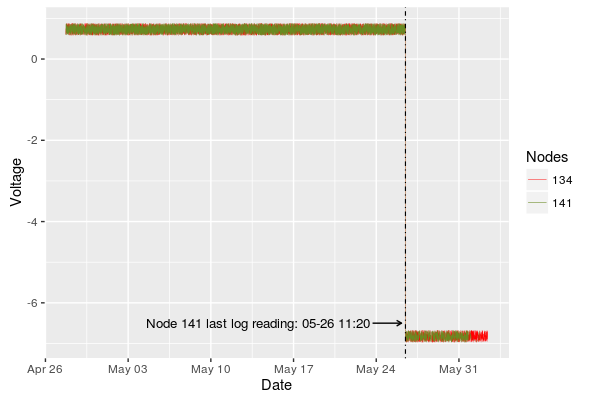
\includegraphics[width=0.9\linewidth]{../figures/voltDate_2.png}
    \caption{Temporal voltage trends: nodes 134 and 141}
    \label{fig:voltDate2}
  \end{subfigure}

  \begin{subfigure}{.5\textwidth}
    \centering
      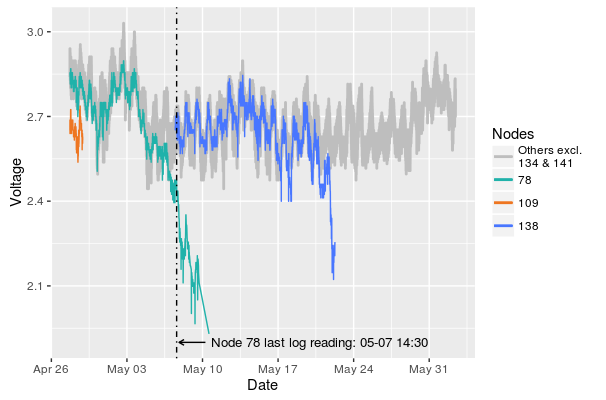
\includegraphics[width=0.9\linewidth]{../figures/voltDate_1.png}
    \caption{Temporal voltage trends:nodes excluding 134 and 141}
    \label{fig:voltDate1}
  \end{subfigure}%
  \begin{subfigure}{.5\textwidth}
    \centering
      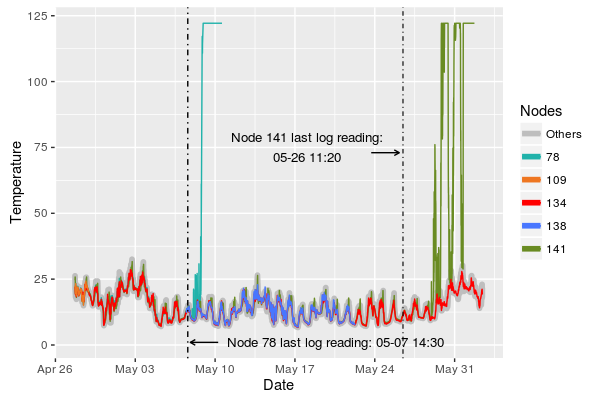
\includegraphics[width=0.9\linewidth]{../figures/tempDate.png}
    \caption{Temporal temperature trends}
    \label{fig:tempDate}
  \end{subfigure}
\caption{Outlier detection by voltage and temperature}
\label{fig:tempVoltOutliers}
\end{figure}%

Figure~\ref{fig:dataCleaning} shows the comparison between the number of the data points from the interior tree before and after data cleaning. Note that the data points from some height levels were all removed, i.e. those at the height of 42, 44.9, 49.6, 49.8, 50, 54, 54.5 and 55.2, because they were deployed outside the experiment envelope.
\begin{figure}[!htb]
  \centering
    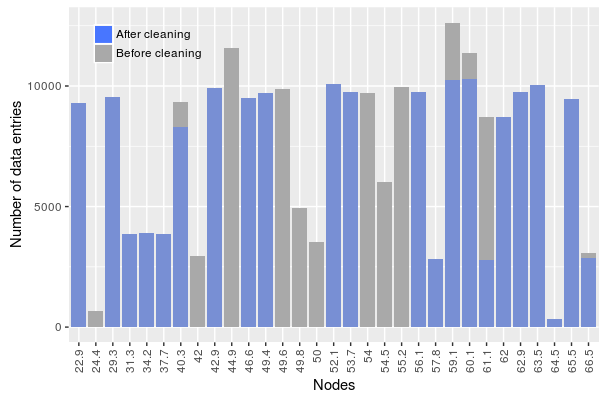
\includegraphics[width=0.5\textwidth]{../figures/dataCleaning.png}
  \caption{Data preservation after cleaning (interior tree)}
  \label{fig:dataCleaning}
\end{figure}


\subsection{Data Exploration}
\subsubsection{Distribution of observations}
To get a general sense of the distribution of the cleaned data, Figure~\ref{fig:distHeight} and Figure~\ref{fig:distDirec} show the histogram of the observations each day, colored in height and direction respectively. Firstly, most of the data were obtained from the nodes deployed to the west side of the trunk before the east node died on May 12th. Secondly, May 7th, May 11th and May 26th are three worth-noting dates as indicated by the three vertical dotted lines. May 7th was the start recording date of the net dataset, and May 26th was when the local data loggers of most nodes were filled up. Since then, the data entry number was almost half as the beginning. May 11th was when the number of observations started to drop, which might be due to battery run-out. Figure~\ref{fig:lifeHeight} shows the life of each node, corresponding to each height level, colored in direction. Only one node was deployed on the east. This deployment bias was intentional by the researchers for the reason described in the previous section, which should be born in mind in further data analysis.
\begin{figure}[here]
\centering
\begin{subfigure}{.5\textwidth}
  \centering
  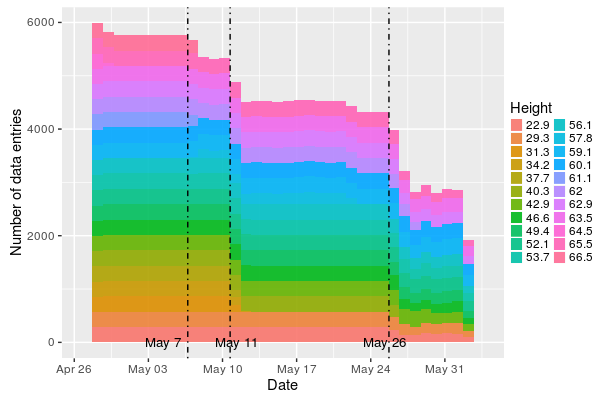
\includegraphics[width=1\linewidth]{../figures/distHeight.png}
  \caption{Data counts per day (colored in Height)}
  \label{fig:distHeight}
\end{subfigure}%
\begin{subfigure}{.5\textwidth}
  \centering
  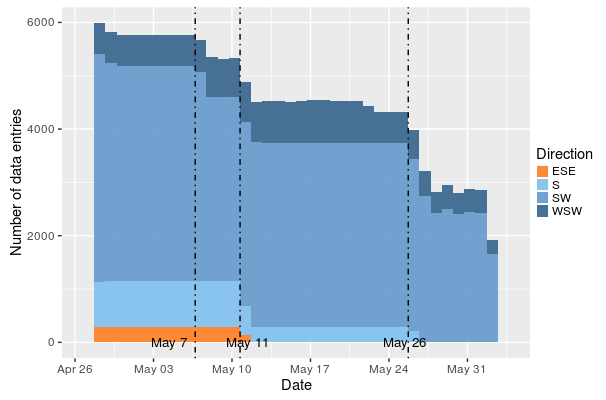
\includegraphics[width=1\linewidth]{../figures/distDirec.png}
  \caption{Data counts per day (colored in Direction)}
  \label{fig:distDirec}
\end{subfigure}
\null \vspace{2em}
\begin{subfigure}{1\textwidth}
  \centering
  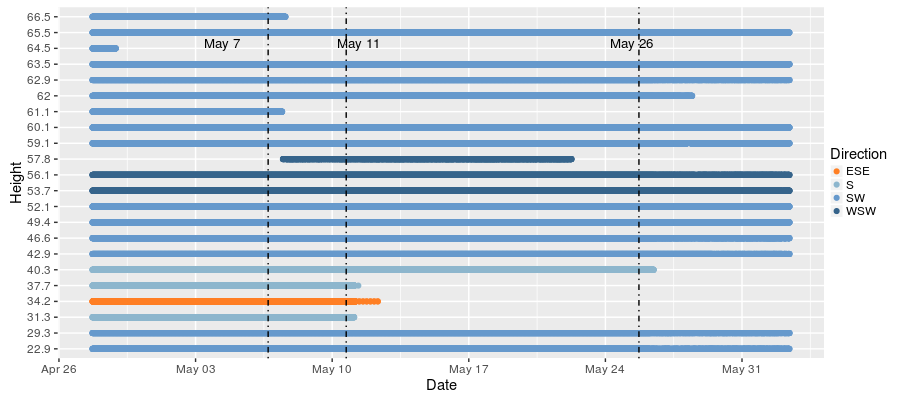
\includegraphics[width=1\linewidth]{../figures/lifeHeight.png}
  \caption{Life of each node}
  \label{fig:lifeHeight}
\end{subfigure}
\caption{Distribution of observations}
\end{figure}
\pagebreak


\subsubsection{Temporal trends of all nodes}
\label{subsubsec:trendAllNodes}
To study what was special about the date May 11th,  a comparison between the temporal data of the four variables on May 11th and on May 1st was drawn. May 1st, as chosen by the original paper, recorded data with most nodes and variance in the four variables. My initial hypothesis about the drop in the data points on May 11th was that some erratical climatic event such as a storm, which should have been captured by temperature or humidity, caused the death of some batteries. \\
The left panel of Figure~\ref{fig:comp111} shows the above comparison and displays a very distinct difference in the data on the two days. For temperature, higher nodes generally recorded higher temperature than the lower ones on May 1st, whereas higher nodes mostly recorded lower temperature on May 11th before a reverse at 17:00. Besides, the variance of temperature was smaller on May 11th than on May 1st. For adjusted relative humidity, similar phenomenon was observed. On May 1st, the upper part of the tree was in general less humid than the lower part, whereas on May 11th, the upper and the lower part were exposed to similar humidity level. However, it was obvious that the entire tree had a higher humidity exposure on May 11th than on May 1st. Hence, it could be inferred that it was sunny on May 1st while foggy or perhaps even rainy on May 11th.\\
It seemingly follows that high humidity level on May 11th caused some batteries to die. However, the claim was disapproved when the data from the two dates were put into the entire deployment window, as shown in the right panel of Figure~\ref{fig:comp111}. The high humidity level on May 11th was not an outlier from the readings in its week. An investigation into the temporal trend of weekly averages was naturally suggested by this graph, which is addressed in section~\ref{subsec:firstFind} later. Additionally, there seems to be a negative correlation between temperature and humidity, across heights and dates. This relationship is also studied later in section~\ref{subsec:thirdFind}.\\
\begin{figure}[!hbt]
  \centering
    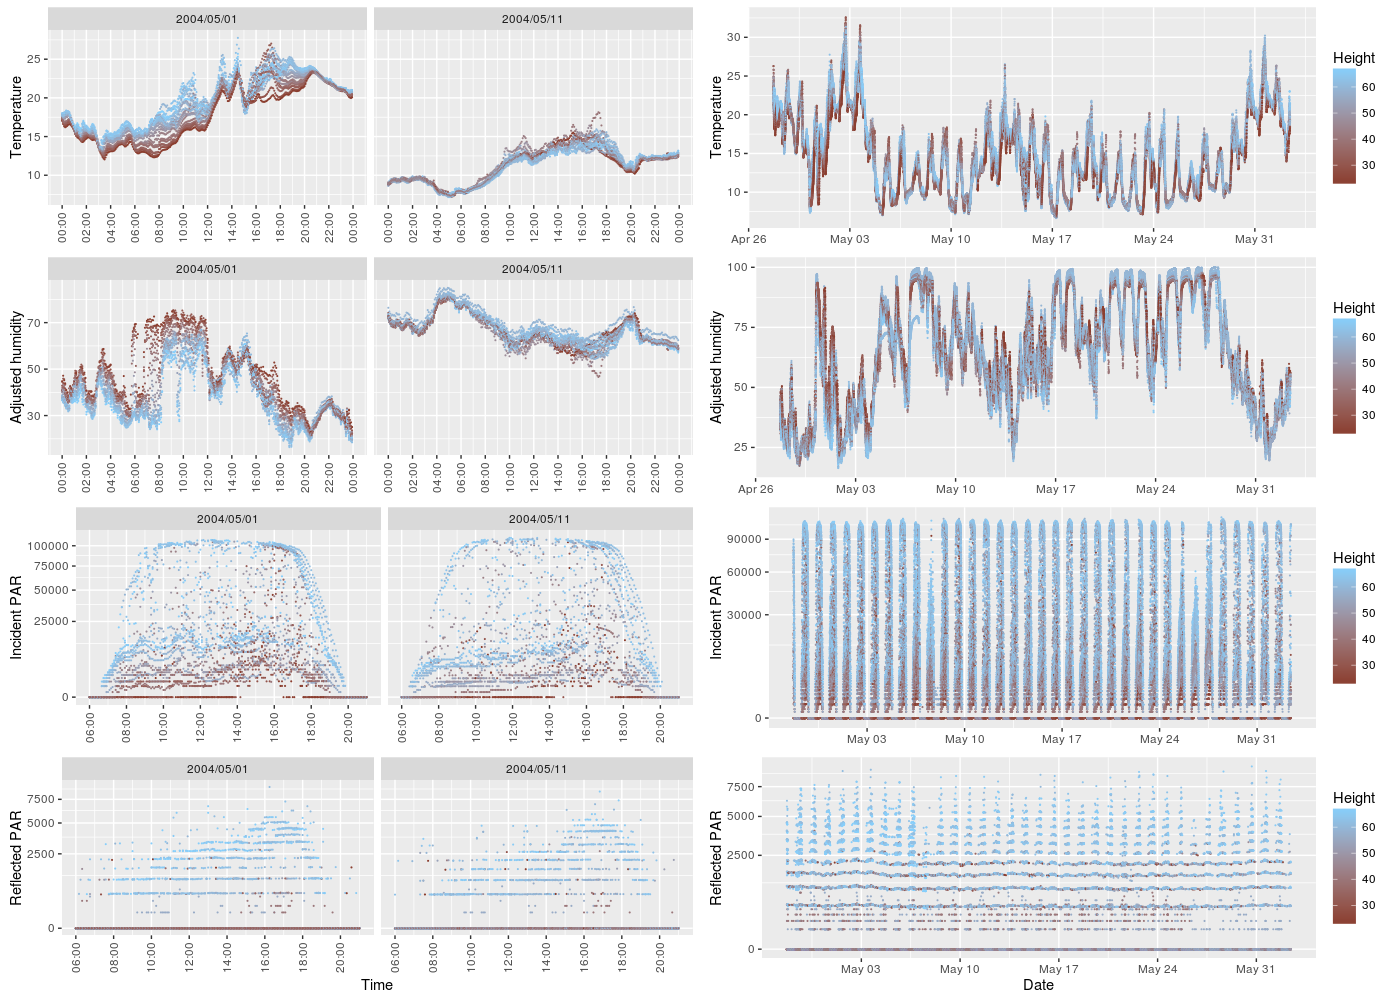
\includegraphics[width=1\textwidth]{../figures/comp111.png}
  \caption{Temporal data on May 1st and 11th (\textit{Left}) and over the entire period (\textit{Right})}
  \label{fig:comp111}
\end{figure}


\subsubsection{Hourly trends of average spatial gradients}
\label{subsubsec:tempSpatial}
The four variable values at each time point were averaged over days in order to observe the temporal movement of spatial gradients. Figure~\ref{fig:avgTemporal} plots time on the horizontal axis, height on the vertical axis, and the magnitude of the readings with color.\\
The upper two plots of Figure~\ref{fig:avgTemporal} show the average movements of temperature and relative humidity throughout the day. Temperature generally peaks in the afternoon when humidity experiences valley. Specifically, as the sun rises at around 06:00, the top of the tree starts to warm up and dry, and then the lower part experiences similar movement in readings until the sun sets at around 20:00, when the lower part of the tree starts to cool down and humidify, followed by the upper part. \\
The same applies to the sunlight readings shown in the lower two plots of Figure~\ref{fig:avgTemporal}. Both incident PAR and reflected PAR clearly show the movement of the sun over the period, generally rising at around 06:00 while setting at around 20:00. The peak illumination in the afternoon can be accounted by the fact that most of the nodes were deployed to the west side of the trunk. \\
The plots show that the top usually led any movement in readings. This is attributed to the buffering effect of the thick canopy on the lower west side. Hence, the upper part of the tree expenrienced larger variance in all microclimatic measures than the lower part within the same distance to the trunk. One might deduce that a node placed outside the deployment range, hence without the shield from the canopy, might have experienced larger variance.
\begin{figure}[!h]
  \centering
    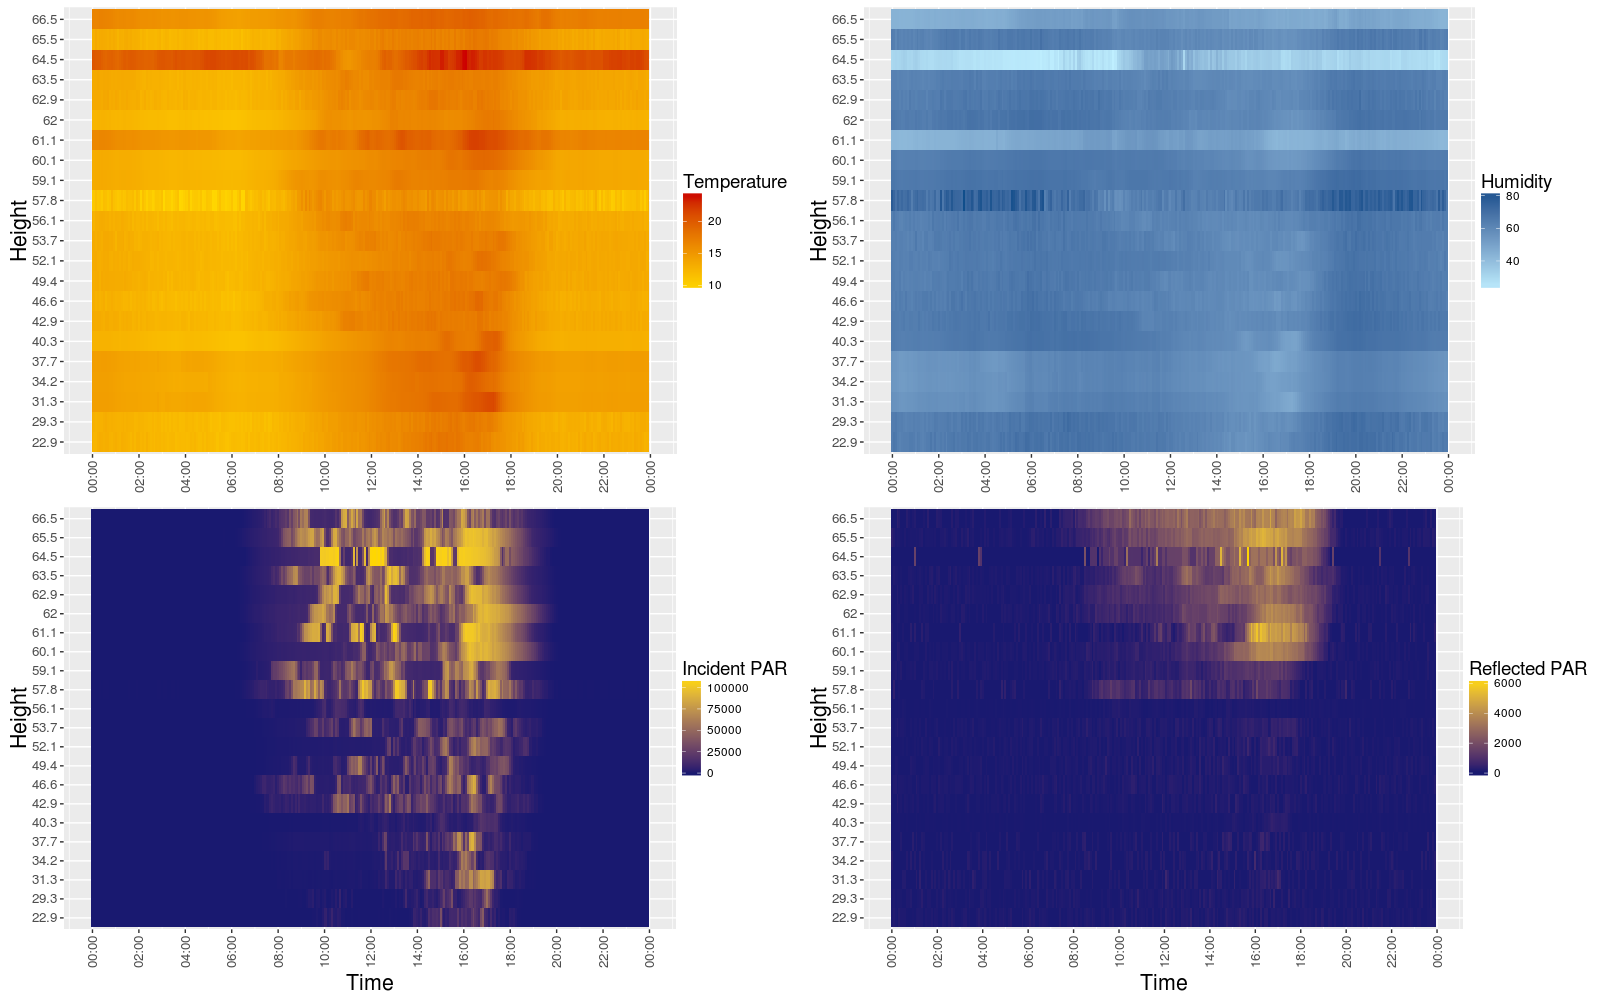
\includegraphics[width=.9\textwidth]{../figures/avgTemporal.png}
  \caption{Temporal trends of spatial gradients}
  \label{fig:avgTemporal}
\end{figure}

\section{Graphical Critique}
\subsection{Critique on Figure 3}
The Figure 3(a) gives an overview of each variable in histograms, and the text briefly describes the distributions and the intuition behind. However, it fails to reason a high proportion of low values for either incident or reflected PAR, around 78\% and 88\% respectively, which is inproportional to the long day time during the deployment envelope. Besides, it would have been more relevant to focus only on PAR values collected during the day while discarding those during the night when the values are 0.\\
The Figure 3(b) summarises the distribution of each variable in a boxplot per day throughout the envolope mixing spatial effects. There are mainly two problems in the figure. Firstly, the data collected in the week of June 3rd should have been discarded because they were biased towards the three nodes mentioned before in section~\ref{subsubsec:preprocess}. Secondly, due to the high proportions of low PAR values, the boxplots contain mainly outliers, and hence are not informative. An alternative could be plotting the boxplots with night-time values removed for each day.\\
The Figure 3(c) summarises the distribution of each variable in a boxplot per height level mixing temporal effects, and hence is not as informative as 3(d), which reduces time influence by centering the daily values for each variable. The PAR subplots clearly convey the message that lower-level nodes received less light than the higher ones, whether incident or reflected. However, the text hastily claimed that the lower nodes were colder than the higher ones on average, but there was no statistical test or obvious pattern in the temperature subplot.  
\subsection{Critique on Figure 4}
Figure 4 adds time and space information to the variable values on May 1st, when it was claimed to have the widest variation range for each variable. The left panel of the graph shows the temporal trends of all nodes throughout the day, and the right panel shows the spatial gradient at the moment when RH changed drastically for all the nodes. The figure tries to present a 3D picture of the surrounding microclamatic environment surrounding the tree in a 2D setting. However, there was room for improvement. Firstly, the legend should be added along side with the graph, for both the time series data and the spatial data. Secondly, it is also redundant to use both color and orientation of a triangle in the right panel to distinguish the nodes deployed on the west from the east side of the trunk. Figure 5 combines the two panels to show the temporal movement of spatial gradients on May 1st. Additionally, data from the nodes deployed outside the deployment envelope, i.e. those on the east side of the trunk, should be removed from analysis.
\section{Findings}


\subsection{First finding}
\label{subsec:firstFind}
\begin{figure}[!h]
  \centering
    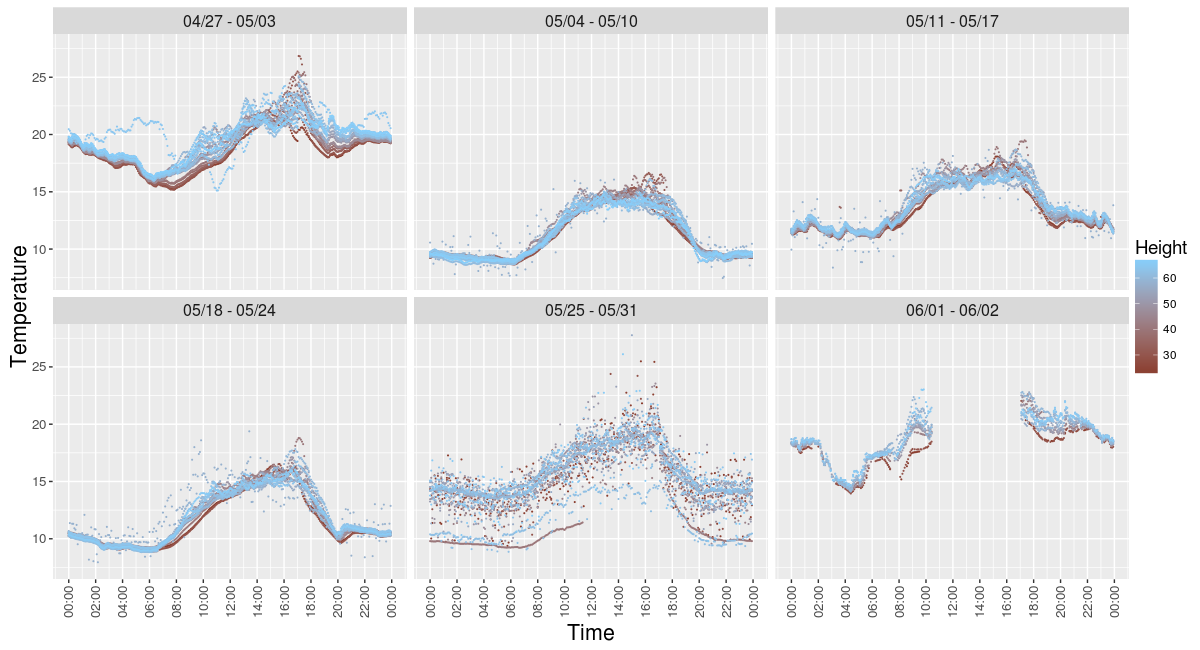
\includegraphics[width=.9\textwidth, height=.42\textwidth]{../figures/tempTemporal.png}
  \caption{Temporal trends of spatial gradients in \textit{Temperature} (colored in \textit{Height})}
  \label{fig:tempTemporal}
\end{figure}
\begin{figure}[!h]
  \centering
    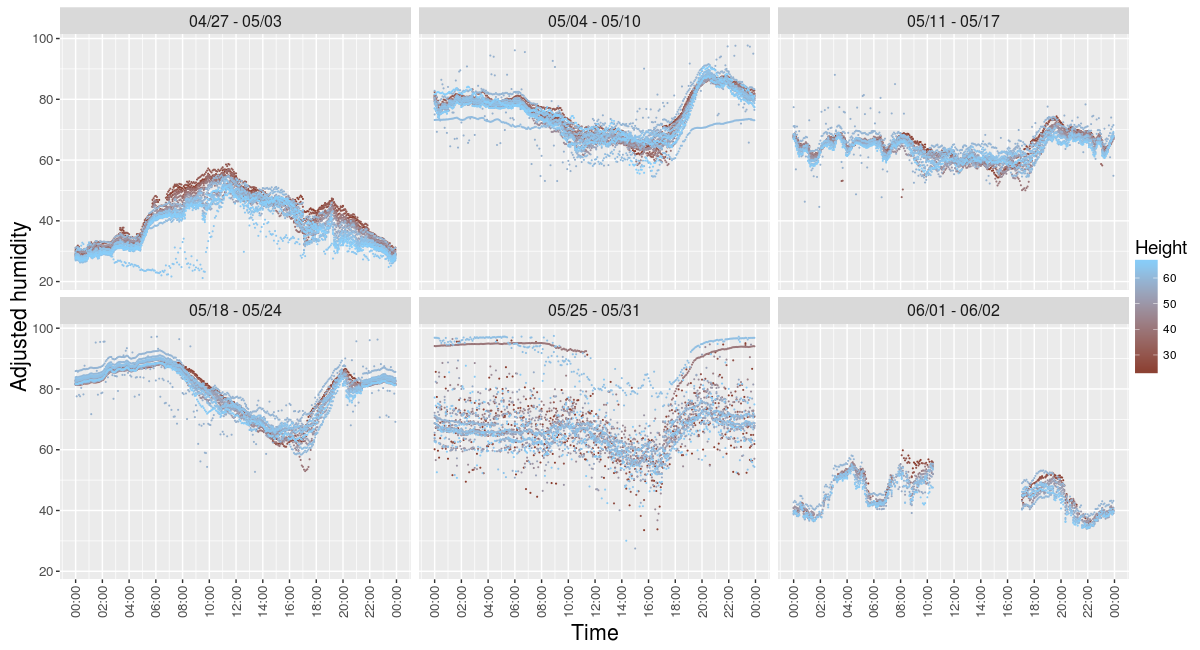
\includegraphics[width=.9\textwidth, height=.42\textwidth]{../figures/humidTemporal.png}
  \caption{Temporal trends of spatial gradients \textit{Adjusted humidity} (colored in \textit{Height})}
  \label{fig:humidTemporal}
\end{figure}
Motivated in Subsection~\ref{subsubsec:tempSpatial}, the data were averaged at each time point on a weekly basis instead of over the entire deployment period. Note that because of data incompleteness in the later period both due to data logger memory fill-up and network failure, the data saw larger variance in the week May 25 to May 31 and missing values for the noon time during the last two days. They were plotted seperately instead of combined with data from other weeks to avoid visual bias.\\
Figure~\ref{fig:tempTemporal} shows clearly that the upper of tree was generally warmer than the lower part, but in the afternoon near dawn, the lower part was almost as warm as the upper. Also, the upper part warmed up earlier while cooled down later than the lower part in each of the week. Additionally, the variance in temperature was smaller during the night than during the day across heights.\\
Figure~\ref{fig:humidTemporal} shows clearly that the upper was generally less humid than the lower. Interestingly, the first week saw a different trend from the rest. In the first week, the humidity level increased at first until noon when it started to fall, whereas in the rest weeks, the humidity level usually decreased at first until the afternoon when it started to climb up.\\
Combining the two plots, one might deduce a different weather picture for each week. Week 1 was generally warm and dry, the middle three weeks were generally cool and humid, and it went back warm and dry in the last two weeks. Besides, similar to Subsection~\ref{subsubsec:trendAllNodes}, a negative correlation between the two variables was quite obvious.



\subsection{Second finding}
\label{subsec:secondFind}
\begin{figure}[!h]
  \centering
    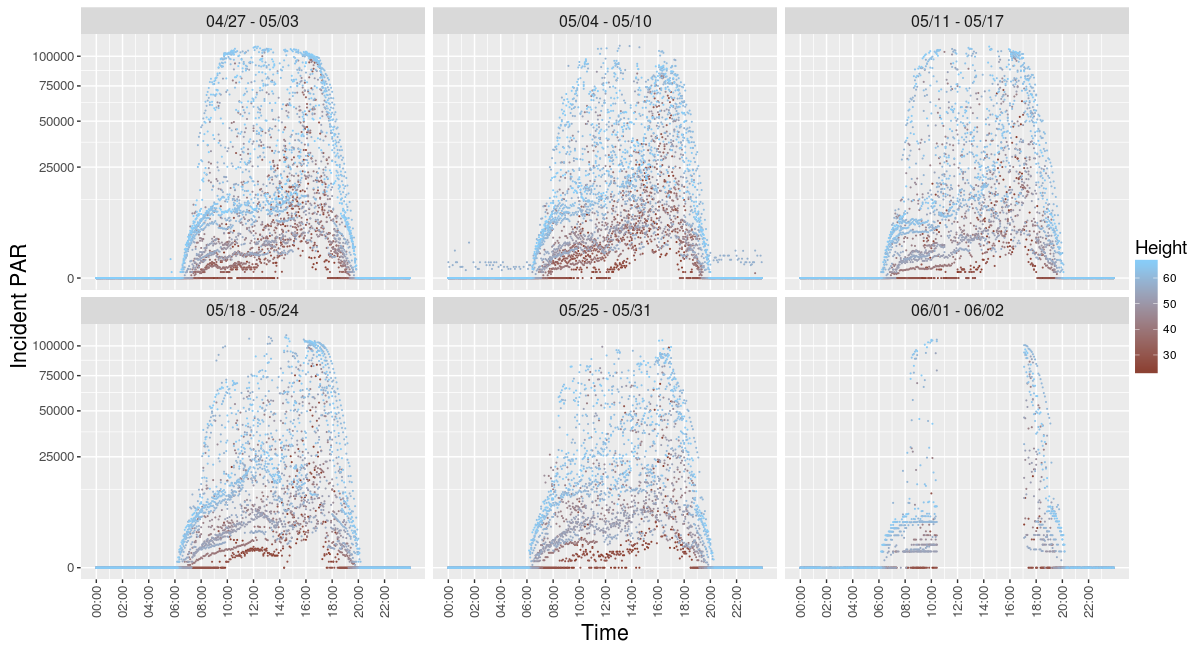
\includegraphics[width=.9\textwidth, height=.42\textwidth]{../figures/iparTemporal.png}
  \caption{Temporal trends of spatial gradients in \textit{Incident PAR} (colored in \textit{Height})}
  \label{fig:iparTemporal}
\end{figure}
\begin{figure}[!h]
  \centering
    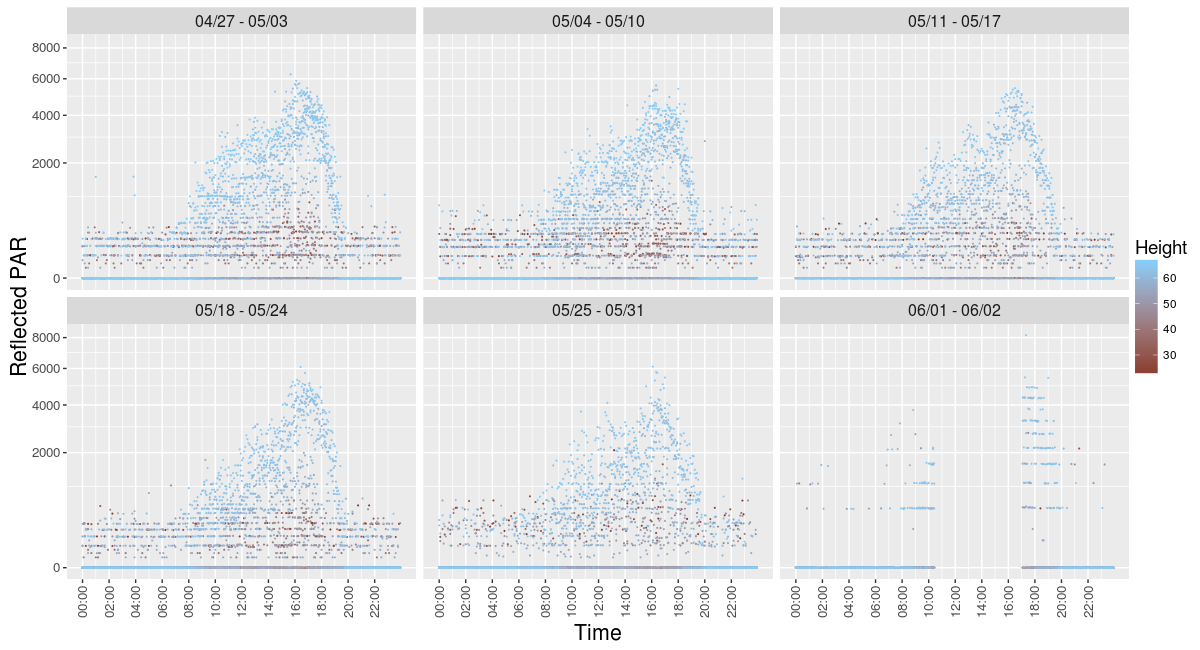
\includegraphics[width=.9\textwidth, height=.42\textwidth]{../figures/rparTemporal.png}
  \caption{Temporal trends of spatial gradients in \textit{Reflected PAR} (colored in \textit{Height})}
  \label{fig:rparTemporal}
\end{figure}
The incident PAR plotted in Figure~\ref{fig:iparTemporal} clearly shows the normal movements of the sun for each week. Particularly, since the nodes were mostly deployed to the west of the trunk, the lower part was exposed to more or less the same level of incident solar radiation as the upper part. However, due to a thicker canopy at the lower tree level, less reflected solar radiation was received by the lower part than the upper. The peak of reflected solar radiation can be attributed to the west-side-deployment of the nodes.

\subsection{Third finding}
\label{subsec:thirdFind}
The relationship between the variables was studied based on a sample of 10,000. \textbf{Stratified sampling} was performed to ensure the sample was representative of the entire dataset, and the correlation between any pair of primary variables was preserved as shown by Figure~\ref{fig:correlation}.
\begin{figure}[!htb]
\centering
\begin{subfigure}{.5\textwidth}
  \centering
  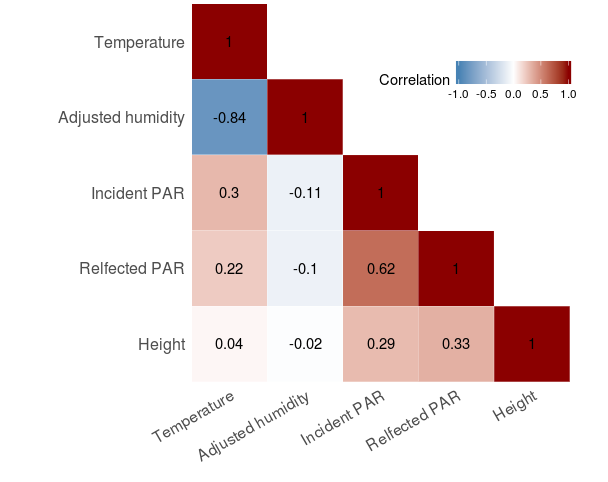
\includegraphics[width=.8\linewidth]{../figures/corrAll.png}
  \caption{The entire dataset}
\end{subfigure}%
\begin{subfigure}{.5\textwidth}
  \centering
  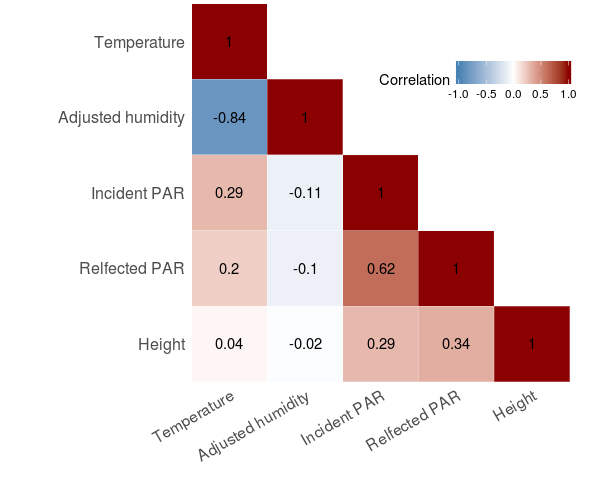
\includegraphics[width=.8\linewidth]{../figures/corrSample.png}
  \caption{The sample of size 10,000}
\end{subfigure}
\caption{Correlation structure between primary variables}
\label{fig:correlation}
\end{figure}

As motivated by the reverse movements of adjusted humidity to temperature shown in Subsection~\ref{subsubsec:trendAllNodes}, the relationship between the two variables is worth studying. Figure~\ref{fig:correlation} notes the correlation between the two variables is -0.84 across throughout the time, and it was calculated that the correlation was -0.82 for the daytime and -0.90 for the night. 
\begin{figure}[!h]
  \centering
    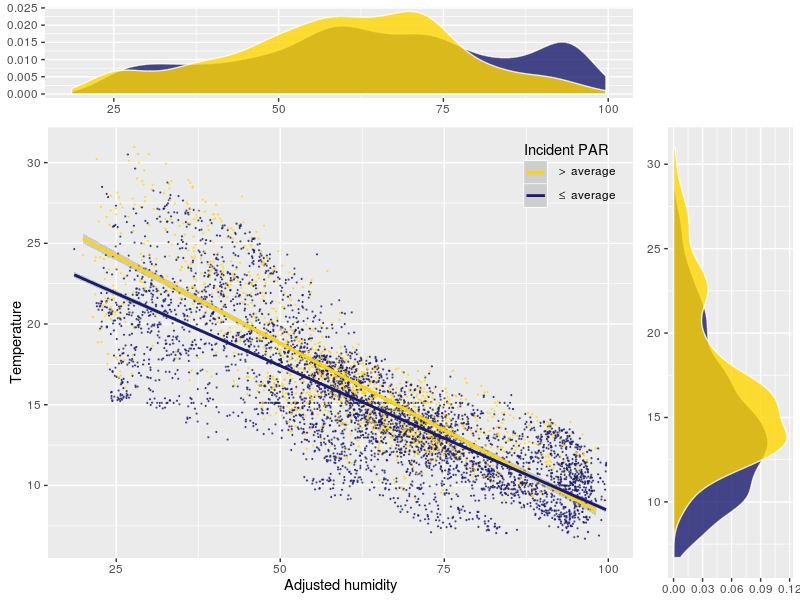
\includegraphics[width=.8\textwidth]{../figures/tmp.png}
  \caption{Temperature vs. adjusted humidity (colored in \textit{Incident PAR})}
  \label{fig:tempHumidPar}
\end{figure}
Similarly, the correlations were slightly different after the data was split into two, one with incident PAR readings below the average and the other above. The below-average group has a correlation of -0.85 and the other -0.83. Figure~\ref{fig:tempHumidPar} plots such a relationship, colored in the two incident PAR level groups. Seeing the above-average group has a steeper regression line than the below-average, it is deduced that the ratio of the sample variance of temperature to that of adjusted humidiy was larger for the above-average group. In other words, the higher level of solar radiation the tree part was exposed to, the more the temperature level varied compared to the humidity level. Since the higher part of the tree in general was exposed to higher level of solar radiation, it follows that the higher part should have a larger variance in temperature and a smaller one in humidity, which is consistent with the Finding~\ref{subsec:firstFind}.\\
\begin{figure}[!htb]
\centering
\begin{subfigure}{.5\textwidth}
  \centering
  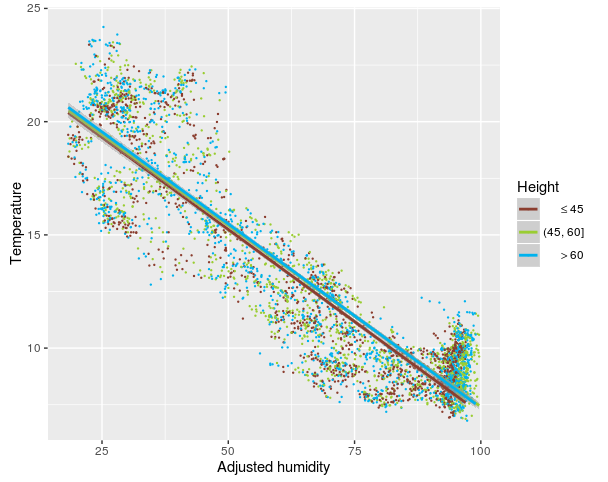
\includegraphics[width=.9\linewidth]{../figures/tempHumidHeightall.png}
  \caption{During both day and night}
  \label{fig:thhall}
\end{subfigure}%
\begin{subfigure}{.5\textwidth}
  \centering
  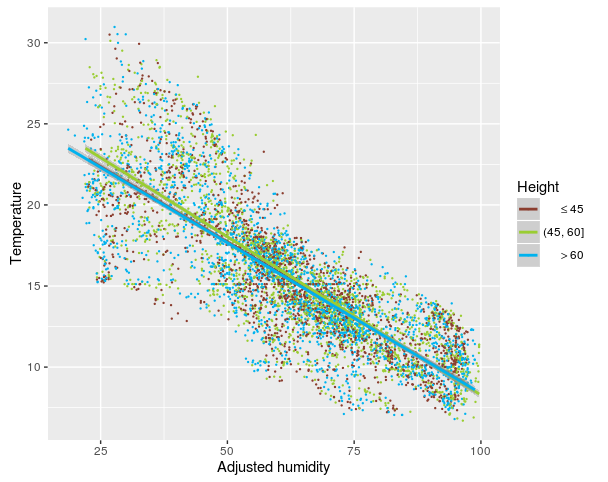
\includegraphics[width=.9\linewidth]{../figures/tempHumidHeightday.png}
  \caption{Only during the day}
  \label{fig:thhsample}
\end{subfigure}
\caption{Temperature vs. adjusted humidity (colored in \textit{Height})}
\label{fig:tempHumidAllDay}
\end{figure}
However, there is no obvious difference in height groups, be it for the whole time or only for the day time. Figure~\ref{fig:thhall} shows the relationship for the data during both day and night, whereas Figure~\ref{fig:thhsample} shows the relationship only based on the data during the day.


\section{Discussion}
Limited by page and time constraints, the report revolves around the data obtained from the nodes deployed within a deployment envelope from the interior tree. More analysis could have been done on both the nodes outside the deployment envelope of the interior tree and the nodes deployed on the edge tree. A comparison between the two might reveal some interesting patterns in microclimatic dynamics within different parts of a woods. However, exploratory data analysis seems to be the most one can perform in lack of developed biological models describing dynamics between microclimatic variables. Lack of valuable data points towards the end of the experiment period due to such reasons as battery run-out, memory exhaustion and network failure also weighed on analysis and could have biased the results.

\section{Conclusion}
The report details an alternative method to clean and adjust the original dataset, exhaustively explores relationships among the primary variables and presents interesting findings in the last section. Much of the analysis of the microclimatic dynamics would have been impossible withou the development of wireless sensors over a large physical volume.

\section*{Acknowledgments}
Acknowlegements are given to Siyao Chang, Chih-Hui Wang and Tianyi Zhang for valuable discussion on various data cleaning and analysis ideas.

\bibliographystyle{plain}
\bibliography{sensor}

\end{document}
